\documentclass[10pt]{jsarticle}
\usepackage{braket}
\usepackage[dvipdfmx]{graphicx}
\usepackage{bm}

\newcommand{\pref}[1]{(\ref{#1})}
\newcommand{\ope}[1]{\hat{#1}}
\newcommand{\normord}[1]{\mathopen{:}#1\mathclose{:}}
\newcommand{\prob}{p}
\newcommand{\Prob}{P}
\newcommand{\dist}{Q}
\newtheorem{definition}{定義}
\renewcommand{\thedefinition}{}
\newtheorem{theorem}{定理}
\renewcommand{\thetheorem}{}

\title{レーザー光の量子状態とホモダイン測定}
\author{川久保亮}
\date{平成21年2月}

\begin{document}

\maketitle

\begin{abstract}
  この文章は\texttt{jsarticle}を使ったサンプル文書です。既存の文書の内容を大
  幅に改変しているため、内容は信用しないでください。
\end{abstract}

\section{序論}

量子論は二十世紀初頭から発達を始め、電子や光子などの振る舞いを記述する理論として、
素粒子論から物性理論にいたるまで非常に広範囲にわたって影響を与えた。その正当性は、
古典物理学からは考えられないような様々な現象の観測を通して強力に裏付けられている。

量子論の持つユニークな特徴として、重ね合わせの原理と測定による状態の射影が挙げら
れる。量子論的な重ね合わせは環境からのノイズに弱く、直接実験的に観測することは長
く困難であった。しかし近年様々な実験技術の向上によって、原子や光子の重ね合わせ状
態を直接制御、観測することが可能となってきている。このことによって、物理系に対す
る操作や観測を記述する際に測定による射影効果を正しく取り入れることの重要性が増し
ている。\footnote{これは脚注の例です。これは脚注の例です。これは脚注の例です。
これは脚注の例です。これは脚注の例です。これは脚注の例です。}

この流れに伴って、量子論の本質的な性質を検証するような研究や、そのような性質に基
づいた量子通信や量子計算といった新しい技術についての研究が盛んに行われている。こ
のような研究においては、量子論的な性質を顕著に示す光が重要な役割を果たしている。
特に量子通信については、光が唯一の実現手段と言っても過言ではない。光を用いて量子
計算を行う方法も多数提案され、精力的に研究されている。

光を用いた研究を行う際、最も重要なデバイスはレーザーである。レーザーは共振器内部
の媒質による誘導放出を利用した光源であり、高い単色性や指向性を実現できるため非常
に幅広い分野において利用されている。

レーザーの光は干渉性が高く、独立なレーザー光同士が1次の干渉を示すことが実験的に実
証されている\cite{Magyar1963}。光の干渉は通常、光の強度に対応する可観測量の期待値
を使って記述される。このような枠組みでは、光の量子状態が光子数状態である時は1次の
干渉は起こらず、1次の干渉があるためには光が光子数状態の重ね合わせ状態になっていな
ければならない。そのため一般的には、レーザーの光の量子状態は光子数状態の重ね合わ
せ状態であるコヒーレント状態とされている。

ところがM{\o}lmerは、レーザーの発振機構からはコヒーレント状態は生成され得ず、真
の状態は光子数状態の混合状態になっているとした。また、光の状態が光子数状態である
場合でも、測定による射影効果を考えることで1次の干渉を記述できることを直観的に示
した\cite{Molmer1997}。

M{\o}lmerによるこの結果は多くの議論を呼んだ。特に、光子数状態の重ね合わせ(コヒー
レンス)がない場合は真の連続変数量子テレポーテーションは不可能であるとの指摘が
Rudolphらによってなされた\cite{Rudolph2001}。また、レーザー光の量子状態がコヒー
レント状態でないのならば、コヒーレント状態の干渉を用いた測定法の一つであるホモダ
イン測定も新たに検討し直す必要がある。一方で、コヒーレント状態を用いた従来の理論
が実験との整合性という点で成功をおさめていることも事実である。

そこで本研究では、コヒーレント状態と光子数混合状態の二つの状態を区別することは可
能か、という問題について考える。もし二つの状態を区別できないのであれば、レーザー
光の「真の状態」はどちらかという問いは無意味である。この問題を考えるために、主に
ホモダイン測定を題材として考察を進めていく。

まず第\ref{chap:preparation}章では、上の問題を考える際の予備知識を解説する。第
\ref{chap:localization}章では、van Enkら\cite{vanEnk2002}に従ってレーザー共振器
の外部の量子状態を導いた後、Sandersら\cite{Sanders2003}と同様の手続きを用いて位
相の局在化について考察する。

\section{光の量子状態、光学素子と干渉効果}
\label{chap:preparation}

本章では、レーザー光の量子状態について考察するために必要となる基本的な事項につい
て\cite{Matsuoka,Leonhardt,Vogel}に従って解説する。

\subsection{電磁場の量子化}

レーザー光の量子状態を論じるためには、電磁場を量子化しなければならない。本節では
まず、有界領域中の離散モードの電磁場の量子化を与え、体積を無限大にする極限によっ
て連続モードの場合の量子化を導く。また、一次元的な問題に適した近似である近軸近似
について述べる。

\subsubsection*{近軸近似}
\label{sec:paraxial}

前項では無限空間内で全ての方向の波数成分を持った場を考えたが、光学ではレーザー光
など、有限の断面積を持って一次元的に伝播する場を考えることが多い。$z$軸方向に一
次元的に伝播する波動は$xy$方向に無限の広がりを持った平面波$e^{i(kz-\omega t)}$で
あり、有限の断面積を持ったビームは厳密に一次元的に伝播することはできない。しかし
、細長い共振器から出るビームのように直交方向に小さい波数しか持たない場については、
有限の断面積を持った平面波として近似できる。

\subsection{光の量子状態}
\label{sec:state}


\subsection{光学素子}
\label{sec:device}

本節では通常の光学実験において用いられる基本的な光学素子を必要な範囲で説明する。
具体的には、線型光学素子の位相シフターとビームスプリッターについて述べた後、光検
出器を簡単に説明する\cite{Leonhardt,Vogel}。

\subsubsection*{位相シフター}

光が誘電体中を通過すると、真空中を伝播した場合に対して位相差が付く。また、光路の
長さを変化させた場合も、それに応じて位相が変化する。これらを利用して光の位相を調
整する光学素子が位相シフターである。

\subsubsection*{ビームスプリッター}

前項では位相シフターによる反射は無いものとしており、一つの入力モードに一つの出力
モードが対応している。入射光線に対して誘電体の境界面に角度がある場合、入射光は透
過光と反射光の二つのモードに分けられる。入射の方向を逆転してみれば分かるように、
一般には二つの入力モードに対し二つの出力モードが対応することになる。このような光
学素子をビームスプリッターという。

\section{レーザー光の量子状態と測定による干渉、位相の局在化}
\label{chap:localization}

M{\o}lmerは、レーザー光の量子状態は一般的に受け入れられているコヒーレント状態では
なく、光子数状態のインコヒーレントな混合状態であり、その場合でも測定による射影効
果で1次干渉が見られることを示した\cite{Molmer1997}。本章ではM{\o}lmerの議論を紹介
した後、van Enkら\cite{vanEnk2002}にしたがってレーザー共振器外部の場の量子状態を
導く。次にレーザー光の干渉を考察し、測定によって光の位相が局在化することが本質的
であることを見る。最後に、レーザー光を参照光として用いたホモダイン測定について考
察する。

\subsection{レーザー光の量子状態と干渉}
\label{sec:molmer-interference}

レーザー(laser, \textit{light amplifier by stimulated emission of radiation})は共
振器中の原子の誘導放出を利用した光源であり、高い単色性や指向性を兼ね備えた光源と
して非常に幅広い分野において応用されている。MagyarとMandelによって、独立な二つの
レーザーから出る光が1次の干渉を示すことが実験的に実証されており\cite{Magyar1963}、
レーザー光は高い干渉性を持つコヒーレントな光であるとされている。このような特徴か
ら、レーザーから出た光の量子状態の記述にはコヒーレント状態を用いるのが一般的であ
る。

\begin{figure}[htbp]
  \centering
  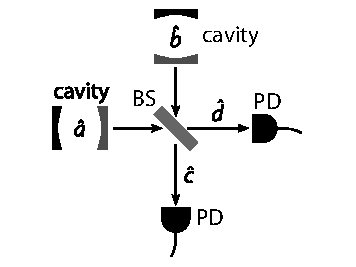
\includegraphics{molmer-interference.pdf}
  \caption{二つの独立なレーザー間の干渉実験の概念図。PDは光検出器、BSはビームス
    プリッターを表す。}
  \label{fig:indep-interference}
\end{figure}

M{\o}lmerはこの問題に対して、検出器による測定の効果を考えることで、光子数状態の重
ね合わせがない場合でも1次の干渉が見られることを数値的に示した\cite{Molmer1997}。
図\ref{fig:indep-interference}のような二つの独立なレーザー間の干渉実験を考える。
二つのレーザー共振器内部の場を消滅演算子$\ope{a}$, $\ope{b}$で表す。これらの場の
周波数は$\omega_a$および$\omega_b$であるとする。共振器から外部に放出された光
は、50:50のビームスプリッターで混合された後二つの検出器で検出される。周波数の
差$\Delta = \omega_a - \omega_b$が0でない場合$\ope{a}$と$\ope{b}$の間には時間に比
例して位相差が付くので、光子の検出数が時間に依存して振動すれば1次の干渉が起きてい
るといえる。

\subsection{レーザー共振器内外の場の定式化}
\label{sec:laser-state}

二つの独立な光子数状態が測定の影響を受けて1次の干渉を示すというM{\o}lmerの結果は、
多くの議論を巻き起こした。特に量子情報分野では2001年にRudolphらが、レーザー光の
ように光子数状態の重ね合わせ(コヒーレンス)を持たない光源では、真の連続変数量子
テレポーテーションは不可能であると主張した\cite{Rudolph2001}。それに対してvan
Enkらは、レーザー共振器の内部と外部の場の関係を考えることで反論を行っ
た\cite{vanEnk2002}。その後Sandersらが、van Enkらと類似の定式化を用いて、光子数状
態同士の干渉を見通し良く定性的に議論した\cite{Sanders2003}。

レーザー光の量子状態がコヒーレンスを持たない場合、従来の干渉の扱いは破たんしてしまう。
したがってそれに依存したホモダイン測定
についても新たに検討し直すことが必要である。また、\ref{sec:molmer-interference}
節で述べたようにコヒーレント状態と光子数混合状態はともに1次の干渉を示すが、これら
二つの状態を実験的に区別することができるかどうかが問題になる。本研究では、まずホ
モダイン測定を題材としてこの問題を検討し、後に一般の測定に拡張する。

\subsubsection*{入力場と出力場の関係}

標準的な入力・出力理論\cite{input-output}を用いて、レーザー共振器内部の場と共振器
から出力される場の関係を導く。\ref{sec:paraxial}節の近軸近似が成り立っている状況
を仮定する。共振器の長さを$L$とし、片側は完全に反射する鏡、片側は減衰率$\kappa$
の半透鏡で構成されているとする。まず、場のモードを二つに分ける。共振器内部の周波
数$\omega_0$の場を消滅演算子$\ope{a}$, 共振器外部の周波数$\omega$の連続モードの場
を消滅演算子$\ope{b}(\omega)$で表す。このようにモードを分けるのは近似であり、
\begin{enumerate}
\item 共振器のフィネスが十分高く、減衰率$\kappa$が共振周波数の間隔$\Delta\omega
  = \pi c/L$より十分小さい
\item 共振器内の光の往復時間$2L/c$に比べて時間スケール$\Delta t$が十分大きい
\end{enumerate}
という条件が満たされている場合に妥当である\cite{Vogel}。

\section{まとめ}

本研究では、レーザー光の量子状態の記述を巡る問題について、ホモダイン測定を題材と
して検討した。まずvan Enkらにしたがってレーザー共振器内外の場を定式化し、共振器
内部の状態がコヒーレント状態の場合と混合状態の場合とで、共振器外部の場の状態を導
いた。次に、Sandersらと同様の方法を用いて、測定による効果を考慮に入れてホモダイ
ン測定を記述した。その結果、混合状態を参照光として用いる場合でも測定に伴って位相
の局在化が起こり、ある条件下ではコヒーレント状態の場合と等価になることを示した。

本研究の後半では、さらに一般的な場合について考えるために測定の条件付き確率分布を
比較することが必要であることを指摘し、ホモダイン測定の数値シミュレーションを行っ
た。シミュレーションからは、二つの状態が等価であり区別できないことを示唆する結果
が得られた。この結果を踏まえて、確率論におけるde Finettiの定理を問題に適用し、上
記の予想が正しいことを示した。すなわち、コヒーレント状態と混合状態のどちらの状態
を用いても同じ現象を記述することができ、またどのような測定を用いてもこれらの状態
を区別することはできないことが分かった。

\begin{thebibliography}{66}
\bibitem{Matsuoka} 松岡正浩,量子光学(東京大学出版会,1996).
\bibitem{Leonhardt} U. Leonhardt, \textit{Measuring the Quantum State of Light}
  (Cambridge University Press, 1997).
\bibitem{Vogel} W. Vogel and D.-G. Welsch, \textit{Quantum Optics}, 3rd ed.\
  (Wiley-VCH, 2006).
\bibitem{Tyc2004} T. Tyc and B. C. Sanders, J. Phys.\ A \textbf{37}, 7341
  (2004).
\bibitem{Magyar1963} G. Magyar and L. Mandel, Nature \textbf{198}, 255 (1963).
\bibitem{Sargent} M. Sargent, M. O. Scully, and W. E. Lamb, \textit{Laser
    Physics} (Addison Wesley, 1974).
\bibitem{Molmer1997} K. M{\o}lmer, Phys.\ Rev.\ A \textbf{55}, 3195 (1997);
  J. Mod.\ Opt.\ \textbf{44}, 1937 (1997).
\bibitem{Bartlett2006} S. D. Bartlett, T. Rudolph, and R. W. Spekkens, Int.\
  J. Quant.\ Inf.\ \textbf{4}, 17 (2006).
\bibitem{Dalibard1992} J. Dalibard, Y. Castin, and K. M{\o}lmer, Phys.\ Rev.\
  Lett.\ \textbf{68}, 580 (1992); R. Dum, P. Zoller, and H. Ritsch, Phys.\ Rev.\
  A \textbf{45}, 4879 (1992).
\bibitem{Rudolph2001} T. Rudolph and B. C. Sanders, Phys.\ Rev.\ Lett.\
  \textbf{87}, 077903 (2001).
\bibitem{vanEnk2002} S. J. van Enk and C. A. Fuchs, Phys.\ Rev.\ Lett.\
  \textbf{88}, 027902 (2001); arXiv:quant-ph/0111157.
\bibitem{Sanders2003} B. C. Sanders and S. D. Bartlett, T. Rudolph, and
  P. L. Knight, Phys.\ Rev.\ A \textbf{68}, 042329 (2003).
\bibitem{Vaidman1994} L. Vaidman, Phys.\ Rev.\ A \textbf{49}, 1473 (1994).
\bibitem{input-output} D. F. Walls and G. J. Milburn, \textit{Quantum Optics}
  (Springer-Verlag, 1994); C. W. Gardiner and M. J. Collett, Phys.\ Rev.\ A
  \textbf{31}, 3761 (1985).
\bibitem{Blow1990} K. J. Blow, R. Loudon, S. J. D. Phoenix, and T. J. Shepherd,
  Phys.\ Rev.\ A \textbf{42}, 4102 (1990).
\bibitem{tomography} K. Vogel and H. Risken, Phys.\ Rev.\ A \textbf{40}, 2847
  (1989); D. T. Smithey, M. Beck, and M. G. Raymer, Phys.\ Rev.\ Lett.\
  \textbf{70}, 1244 (1993).
\bibitem{Hewitt} E. Hewitt and L. J. Savage, Trans.\ Amer.\ Math.\ Soc.\
  \textbf{80}, 470 (1955).
\bibitem{Nielsen} M. A. Nielsen and I. L. Chuang, \textit{Quantum Computation
    and Quantum Information} (Cambridge University Press, 2000), Chap.\ 2.
\bibitem{Bartlett2007} S. D. Bartlett, T. Rudolph, and R. W. Spekkens, Rev.\
  Mod.\ Phys.\ \textbf{79}, 555 (2007).
\end{thebibliography}

\end{document}
